%% LyX 2.3.4.2 created this file.  For more info, see http://www.lyx.org/.
%% Do not edit unless you really know what you are doing.
\documentclass[english,dvipsnames,aspectratio=169,handout]{beamer}
\usepackage{mathptmx}
\usepackage{eulervm}
\usepackage[T1]{fontenc}
\usepackage[latin9]{inputenc}
\usepackage{babel}
\usepackage{amstext}
\usepackage{amssymb}
\usepackage{graphicx}
\usepackage{ifthen}
\usepackage{xcolor}
\usepackage{xspace}
\usepackage{tikz}
\usetikzlibrary{tikzmark}
\usetikzlibrary{calc}
\usepackage{pgfplots}
%\pgfplotsset{compat=1.17}
\usepackage{booktabs}
\usepackage{xpatch}
\usepackage{multirow}
\usepackage{colortbl}
\usepackage{pgfpages}

\newcommand{\commenteq}[1]{{\color{brown}#1}}
\newcommand{\alarm}[1]{{\color{red}#1}}



\xpatchcmd{\itemize}
  {\def\makelabel}
  {\ifnum\@itemdepth=1\relax
     \setlength\itemsep{2ex}% separation for first level
   \else
     \ifnum\@itemdepth=2\relax
       \setlength\itemsep{1ex}% separation for second level
     \else
       \ifnum\@itemdepth=3\relax
         \setlength\itemsep{0.5ex}% separation for third level
   \fi\fi\fi\def\makelabel
  }
 {}
 {}

\ifx\hypersetup\undefined
  \AtBeginDocument{%
    \hypersetup{unicode=true,pdfusetitle,
 bookmarks=true,bookmarksnumbered=false,bookmarksopen=false,
 breaklinks=false,pdfborder={0 0 0},pdfborderstyle={},backref=false,colorlinks=true,
 allcolors=NYUPurple,urlcolor=LightPurple}
  }
\else
  \hypersetup{unicode=true,pdfusetitle,
 bookmarks=true,bookmarksnumbered=false,bookmarksopen=false,
 breaklinks=false,pdfborder={0 0 0},pdfborderstyle={},backref=false,colorlinks=true,
 allcolors=NYUPurple,urlcolor=LightPurple}
\fi

\makeatletter

%%%%%%%%%%%%%%%%%%%%%%%%%%%%%% LyX specific LaTeX commands.
%% Because html converters don't know tabularnewline
\providecommand{\tabularnewline}{\\}

%%%%%%%%%%%%%%%%%%%%%%%%%%%%%% Textclass specific LaTeX commands.
% this default might be overridden by plain title style
\newcommand\makebeamertitle{\frame{\maketitle}}%
% (ERT) argument for the TOC
\AtBeginDocument{%
  \let\origtableofcontents=\tableofcontents
  \def\tableofcontents{\@ifnextchar[{\origtableofcontents}{\gobbletableofcontents}}
  \def\gobbletableofcontents#1{\origtableofcontents}
}

%%%%%%%%%%%%%%%%%%%%%%%%%%%%%% User specified LaTeX commands.
\usetheme{CambridgeUS} 
\beamertemplatenavigationsymbolsempty


% Set Color ==============================
\definecolor{NYUPurple}{RGB}{87,6,140}
\definecolor{LightPurple}{RGB}{165,11,255}


\setbeamercolor{title}{fg=NYUPurple}
\setbeamercolor{frametitle}{fg=NYUPurple}

\setbeamercolor{background canvas}{fg=NYUPurple, bg=white}
\setbeamercolor{background}{fg=black, bg=NYUPurple}

\setbeamercolor{palette primary}{fg=black, bg=gray!30!white}
\setbeamercolor{palette secondary}{fg=black, bg=gray!20!white}
\setbeamercolor{palette tertiary}{fg=gray!20!white, bg=NYUPurple}

\setbeamertemplate{headline}{}
\setbeamerfont{itemize/enumerate body}{}
\setbeamerfont{itemize/enumerate subbody}{size=\normalsize}

\setbeamercolor{parttitle}{fg=NYUPurple}
\setbeamercolor{sectiontitle}{fg=NYUPurple}
\setbeamercolor{sectionname}{fg=NYUPurple}
\setbeamercolor{section page}{fg=NYUPurple}
%\setbeamercolor{description item}{fg=NYUPurple}
%\setbeamercolor{block title}{fg=NYUPurple}

\setbeamertemplate{blocks}[rounded][shadow=false]
\setbeamercolor{block body}{bg=normal text.bg!90!NYUPurple}
\setbeamercolor{block title}{bg=NYUPurple!30, fg=NYUPurple}



\AtBeginSection[]{
  \begin{frame}
  \vfill
  \centering
\setbeamercolor{section title}{fg=NYUPurple}
 \begin{beamercolorbox}[sep=8pt,center,shadow=true,rounded=true]{title}
    \usebeamerfont{title}\usebeamercolor[fg]{title}\insertsectionhead\par%
  \end{beamercolorbox}
  \vfill
  \end{frame}
}

\makeatother

\setlength{\parskip}{\medskipamount} 

\input ../macros

\begin{document}
\input ../rosenberg-macros

%\setbeameroption{show notes on second screen}

\title[DS-GA 1003]{Forward Stagewise Additive Modeling}
\author{He He}
\date{April 13, 2021}
\institute{CDS, NYU}

\makebeamertitle
\mode<article>{Just in article version}


\section{Gradient Boosting / ``Anyboost''}
\subsection{Motivating example: L2 Boosting}
\begin{frame}{FSAM with squared loss}
\begin{itemize}[<+->]
\item Objective function at $m$'th round:
\[
J(v,h)=\frac{1}{n}\sum_{i=1}^{n}\left(y_{i}-\left[f_{m-1}(x_{i})\underbrace{+v h(x_{i})}_{\text{new piece}}\right]\right)^{2}
\]

\item If $\ch$ is closed under rescaling (i.e. if $h\in\ch$, then $vh\in\ch$
for all $h\in\reals$), then don't need $v$.

\item Take $v=1$ and minimize
\[
J(h)=\frac{1}{n}\sum_{i=1}^{n}\left(\left[\underbrace{y_{i}-f_{m-1}(x_{i})}_{\onslide<+->{\text{residual}}}\right]-h(x_{i})\right)^{2}
\]

\item This is just fitting the residuals with least-squares regression!
\item<.-> Example base hypothesis space: regression stumps.
\end{itemize}
\note[item]{Let's consider FSAM with squared loss a s a motivating example.}
\note[item]{Remember that in each round of FSAM we minimize the empirical risk, which is the average loss on the training data. And we only fit one basis function without changing the previous ones.}
\note[item]{Now, we want to find $h$ in our base hypothesis space that minimizes $J$. First notice that if $\sH$ is closed under rescaling, meaning that if a function is in $\sH$ then its scaled version also belongs to $\sH$. Then we can consider $vh$ as another function $g$. Basically we can ignore $v$ if we assume...}
\note[item]{Now, let's re-arrange the terms. How do we interpret the first term?}
\note[item]{It's the residuals, so minimizing $J$ is equivalent to fit the residuals with squared loss.}
\end{frame}
%
%\begin{frame}{Regression Stumps}
%\begin{itemize}
%\item A \textbf{regression stump }is a regression tree with a single split.
%\item A\textbf{ regression stump }is a function of the form \textbf{$h(x)=a\ind{x_{i}\le c}+b\ind{x_{i}>c}$.}
%\end{itemize}
%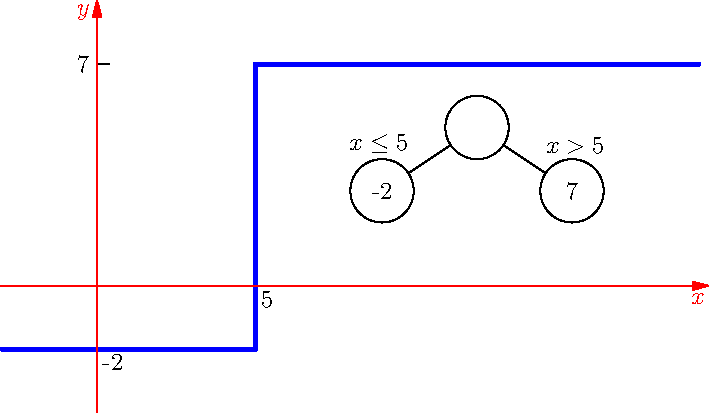
\includegraphics[clip,height=0.7\textheight]{figures/stump}
%\let\thefootnote\relax\footnotetext{\tiny{Plot courtesy of Brett Bernstein.}}
%\end{frame}
%%
\begin{frame}{$L^{2}$ Boosting with Decision Stumps: Demo}
\begin{itemize}
\item Consider FSAM with $L^{2}$ loss (i.e. $L^{2}$ Boosting)
\item For base hypothesis space of \textbf{regression stumps}
\end{itemize}

%\begin{itemize}
%\item Data we'll fit with \href{https://davidrosenberg.github.io/mlcourse/Labs/gbm.py}{code}:
%\end{itemize}
\begin{figure}
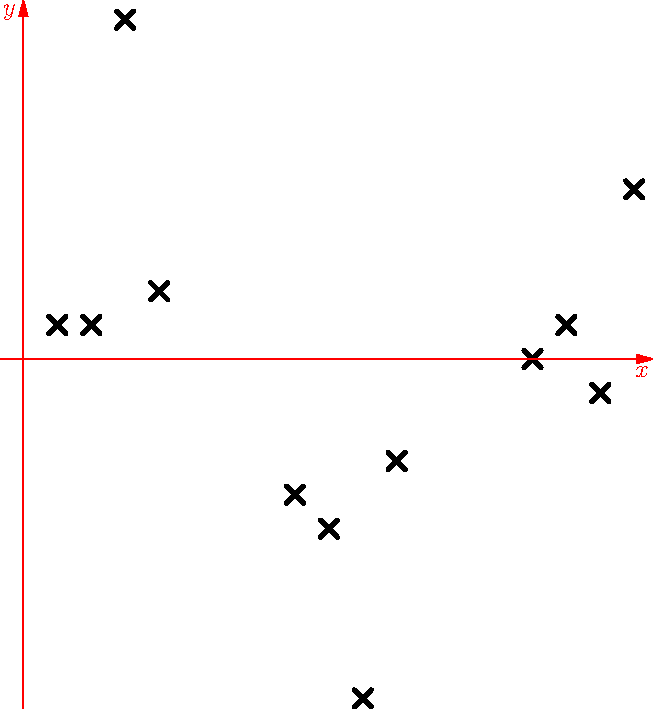
\includegraphics[clip,height=0.6\textheight]{figures/data}
\end{figure}

\let\thefootnote\relax\footnotetext{\tiny{Plot courtesy of Brett Bernstein.}}
\note[item]{Let's look at an example now to go over each round of FSAM with squared loss, which is also called L2 boosting. Our base hypothesis space is regression stumps, which is a regression tree with one split.}
\note[item]{Here's our data. Obviously it's non-linear.}
\end{frame}
%
\begin{frame}{$L^{2}$ Boosting with Decision Stumps: Results}
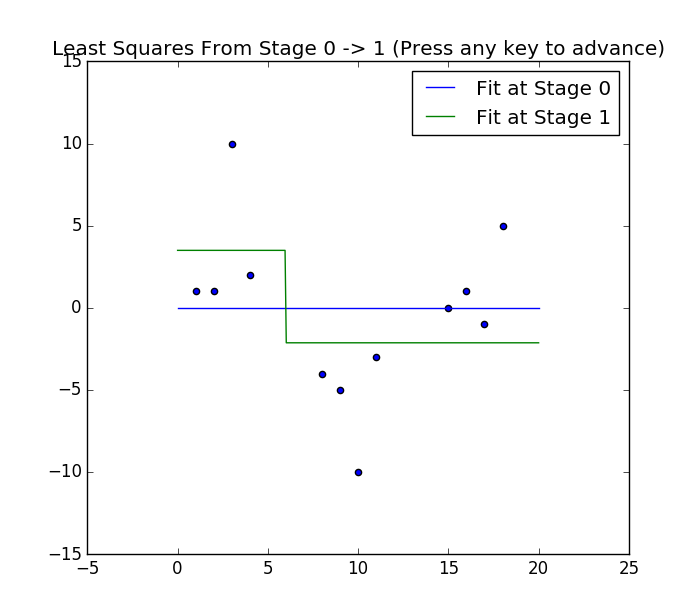
\includegraphics[height=0.8\textheight]{figures/l2boosting-stage1}%
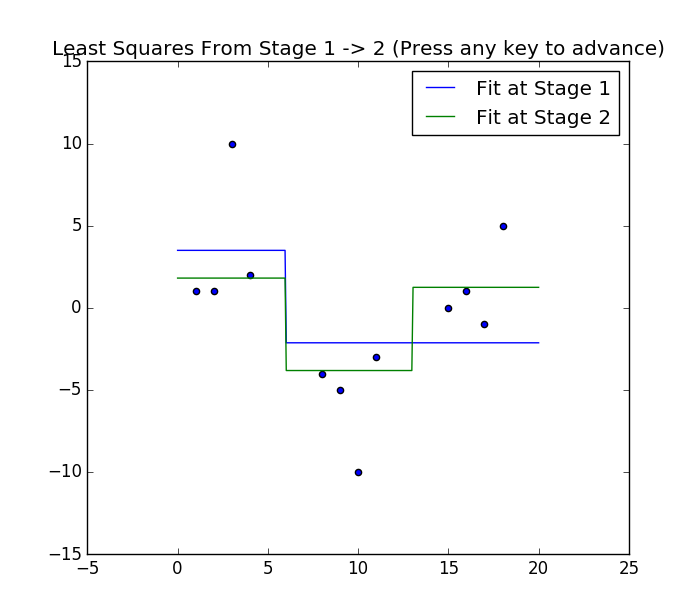
\includegraphics[height=0.8\textheight]{figures/l2boosting-stage2}
\let\thefootnote\relax\footnotetext{\tiny{Plots and code courtesy of Brett Bernstein.}}
\note[item]{Initially, our predictor is constant 0.}
\note[item]{Our first regression stump is the green line.}
\note[item]{In the next stage, we start with the sum of previous predictors, which is the blue line in the right figure.}
\note[item]{We add another decision stump which gives us the green line.}
\end{frame}
%
\begin{frame}{$L^{2}$ Boosting with Decision Stumps: Results}
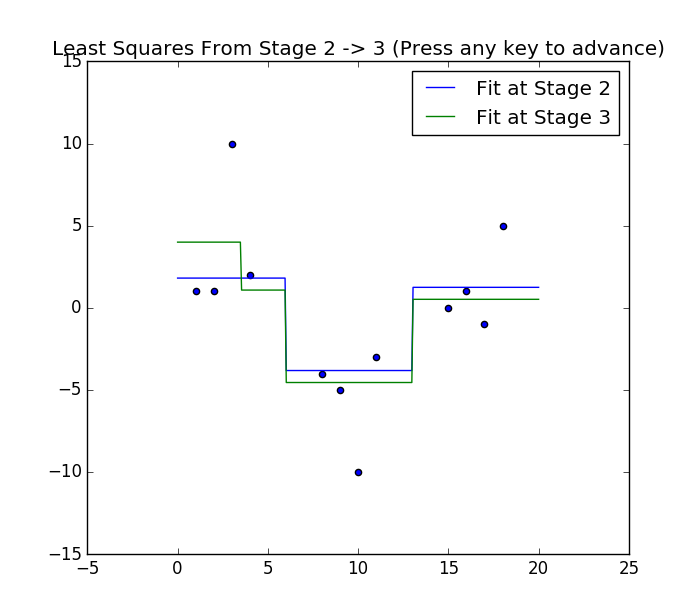
\includegraphics[height=0.8\textheight]{figures/l2boosting-stage3}%
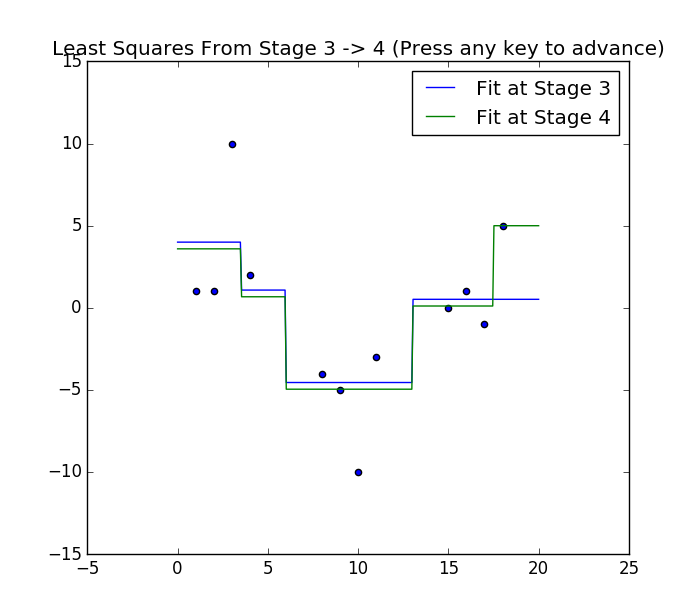
\includegraphics[height=0.8\textheight]{figures/l2boosting-stage4}
\let\thefootnote\relax\footnotetext{\tiny{Plots and code courtesy of Brett Bernstein.}}
\note[item]{So each time we add a new decision stump, so on and so forth.}
\end{frame}
%
\begin{frame}{$L^{2}$ Boosting with Decision Stumps: Results}

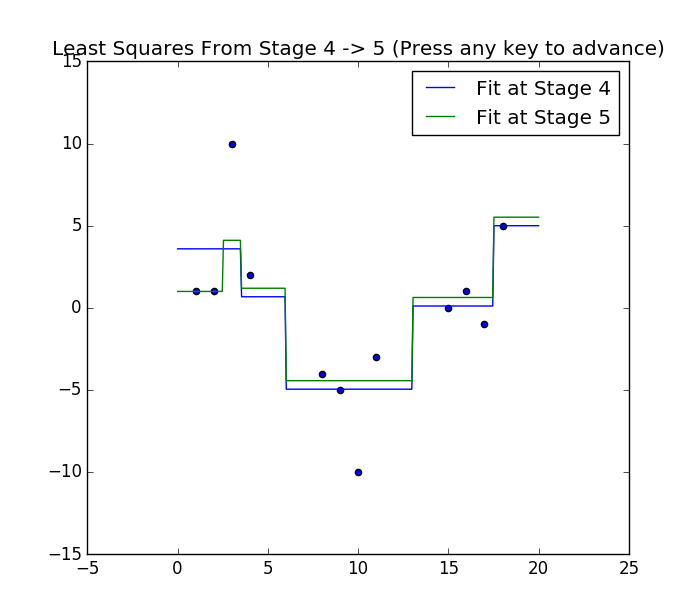
\includegraphics[height=0.8\textheight]{figures/l2boosting-stage5}%
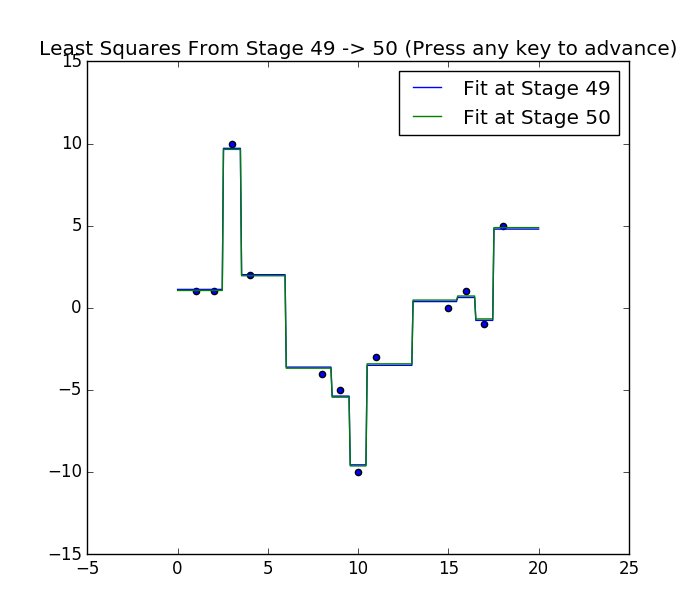
\includegraphics[height=0.8\textheight]{figures/l2boosting-stage50}
\let\thefootnote\relax\footnotetext{\tiny{Plots and code courtesy of Brett Bernstein.}}
\note[item]{After 50 stages, we can see that it overfitted. We will talk about how to prevent overfitting at the end.}
\note[item]{To summarize, in each round, we make a local improvement of our loss function. Specifically, here we move towards the target value incrementally. Now this process is actually quite similar to gradient descent, where we move along the direction that locally minimizes the objective. Next, let's consider its connection to gradient descent in a more formal way.}
\end{frame}

\begin{frame}
{Interpret the residual}
\begin{itemize}[<+->]
\item Objective: $J(f) = \frac{1}{n}\sum_{i=1}^n \p{y_i - f(x_i)}^2 $.
\item What is the residual at $x=x_i$?
\begin{align}
\frac{\partial}{\partial f(x_i)} J(f) = \onslide<+->{ -2 \p{y_i - f(x_i)} }
\end{align}
\begin{itemize}[<.->]
\item Gradient w.r.t. $f$: how should the output of $f$ change to minimize the squared loss.
\item \emph{Residual is the negative gradient} (differ by some constant).
\end{itemize}
\item At each boosting round, we learn a function $h\in\sH$ to fit the residual.
\begin{align}
f &\leftarrow f + {\color{red}v}{\color{Green}h} && \text{FSAM / boosting} \\
\onslide<+->{
f &\leftarrow f - {\color{red}\alpha}{\color{Green}\nabla_f J(f)} && \text{gradient descent}
}
\end{align}
\begin{itemize}[<.->]
\item $h$ approximates the gradient (step direction).
\item $v$ is the step size.
\end{itemize}
\end{itemize}
\note[item]{So this is our loss function. Let's consider the value of $f$ at each training point $x_i$ as a variable that we can optimize.}
\note[item]{Then we can take gradient w.r.t. $f(x_i)$. That means how should we change the output at $x_i$ to minimize $J$.}
\note[item]{In FSAM, in each round we add a weighted basis function.}
\note[item]{Let's compare that with gradient descent. If we consider $f$ as a vector, then in each step, we move the vector along the negative gradient at the current value of $f$.}
\end{frame}

\subsection{Gradient Descent in the Function Space}

%\begin{frame}{FSAM Is Iterative Optimization}
%\begin{itemize}
%\item The FSAM step
%\[
%\left(v_{m},h_{m}\right)=\argmin_{v\in\reals,h\in\ch}\sum_{i=1}^{n}\ell\left(y_{i},f_{m-1}(x_{i})\underbrace{+v h(x_{i})}_{\text{new piece}}\right).
%\]
%
%
%\pause{}
%\item Hard part: finding the \textbf{best} \textbf{step direction} $h$.
%
%\pause{}
%\item What if we looked for the \textbf{locally best }step direction?
%\begin{itemize}
%\item like in gradient descent
%\end{itemize}
%\end{itemize}
%\end{frame}
%%
\begin{frame}{``Functional'' Gradient Descent }
\begin{itemize}
\item We want to minimize
\[
J(f)=\sum_{i=1}^{n}\ell\left(y_{i},f(x_{i})\right).
\]
\item In some sense, we want to take the gradient w.r.t. $f$.

\pause{}
\item $J(f)$ only depends on $f$ at the $n$ training points.

\pause{}
\item Define ``parameters''
\[
{\bf f}=\left(f(x_{1}),\ldots,f(x_{n})\right)^{T}
\]
and write the objective function as 
\[
J({\bf f})=\sum_{i=1}^{n}\ell\left(y_{i,}{\bf f}_{i}\right).
\]
\end{itemize}
\note[item]{We want to minimize $J$ w.r.t. the function $f$ by gradient descent, so the hard part is to compute the gradient, or the step direction.}
\note[item]{Notice that the objective only depends on the value of $f$ at $n$ points and doesn't really care about values elsewhere.}
\note[item]{So let's reformulate the problem by vectorizing $f$ into an $n$-dim vector. Now it becomes a familiar problem---we can easily take gradient w.r.t. this vector $f$.}
\end{frame}
%
\begin{frame}{Functional Gradient Descent: Unconstrained Step Direction}
\begin{itemize}[<+->]
\item Consider gradient descent on 
\[
J({\mathbf{f}})=\sum_{i=1}^{n}\ell\left(y_{i,}{\bf f}_{i}\right).
\]

\item The {negative gradient step direction} at ${\bf f}$ is
\begin{eqnarray*}
-{\bf g} & = & -\del_{\vf}J({\bf f})\\
 & = & -\left(\partial_{{\bf f}_{1}}\ell\left(y_{1},{\bf f}_{1}\right),\ldots,\partial_{{\bf f}_{n}}\ell\left(y_{n},{\bf f}_{n}\right)\right)
\end{eqnarray*}
which we can easily calculate.

\item<.-> $-{\bg}\in\reals^{n}$ is the direction we want to change each of
our $n$ predictions on training data.

\item With gradient descent, our final predictor will be an additive model: $f_0+\sum_{m=1}^M v_t (-\bg_t)$.
\end{itemize}

\note[item]{So what is our gradient now?}
\note[item]{The gradient is simply the vector of partial derivatives w.r.t. $f_i$'s. So now we have the direction towards which we can move our function $f$ at each training points.}
\note[item]{Starting with $f_0=0$, we will get an additive model with gradient descent.}
\end{frame}
%
\begin{frame}{Functional Gradient Descent: Projection Step}
\begin{itemize}[<+->]
\item Unconstrained step direction is
\[
-{\bg}=-\del_{\vf}J({\bf f})=-\left(\partial_{{\bf f}_{1}}\ell\left(y_{1},{\bf f}_{1}\right),\ldots,\partial_{{\bf f}_{n}}\ell\left(y_{n},{\bf f}_{n}\right)\right).
\]
\begin{itemize}[<.->]
\item Also called the ``\textbf{pseudo-residuals}''.
(For squared loss, they're exactly the residuals.)
\end{itemize}

\item 
\alarm{Problem}: only know how to update $\bf$ at $n$ points. How do we take a  gradient step in $\sH$?
\item \emph{Solution}: approximate by the closest base hypothesis $h\in\ch$ (in the $\ell^{2}$ sense):
\begin{align}
\min_{h\in\ch}\sum_{i=1}^{n}\left(-{\bf g}_{i}-h(x_{i})\right)^{2}.
&& \text{least square regression}
\end{align}

\item<.-> Take the $h\in\ch$ that best approximates $-{\bf g}$ as our step
direction.
\end{itemize}
\note[item]{However, our gradient is only defined on $n$ points. In other words, it is in $\reals^n$. But we want an update in the base hypothesis space. In other words, we want to project $g$ to $\sH$.}
\note[item]{So the problem now becomes finding a function in $\sH$ whose values at $x_i$'s are closest to the gradient vector, which is basically a regression problem.}
\end{frame}

\begin{frame}
{Explain by figure}
\note[item]{Draw function fits 1D data. Show the residual and the regression problem.}
\end{frame}

\begin{frame}
{Recap}
\begin{itemize}[<+->]
\item Objective function: 
\begin{align}
J(f) = \sum_{i=1}^n \ell(y_i, f(x_i)) .
\end{align}
\item Unconstrained gradient $\bg \in \reals^n$ w.r.t. ${\vf}=(f(x_1), \ldots, f(x_n))^T$:
\begin{align}
{\bg}=\del_{\vf}J({\bf f})=\left(\partial_{{\bf f}_{1}}\ell\left(y_{1},{\bf f}_{1}\right),\ldots,\partial_{{\bf f}_{n}}\ell\left(y_{n},{\bf f}_{n}\right)\right).
\end{align}
\item Projected negative gradient $h \in \sH$:
\begin{align}
h = \argmin_{h\in\ch}\sum_{i=1}^{n}\left(-{\bf g}_{i}-h(x_{i})\right)^{2}.
\end{align}
\item Gradient descent:
\begin{align}
f \leftarrow f + {\color{red}v}h
\end{align}
\end{itemize}
\note[item]{But we still need to figure out the step size $v$.}
\end{frame}

\begin{frame}{Functional Gradient Descent: hyperparameters}
\begin{itemize}
\item Choose a step size by \textbf{line search}. 
\[
v_{m}=\argmin_{v}\sum_{i=1}^{n}\ell\left\{ y_{i},f_{m-1}(x_{i})+v h_{m}(x_{i})\right\} .
\]
\begin{itemize}
\item Not necessary. Can also choose a fixed hyperparameter $v$.
\end{itemize}
\item Regularization through \textbf{shrinkage}:
\begin{align}
f_m \leftarrow f_{m-1} + {\color{blue}\lambda} v_m h_m \quad \text{where}\; \lambda \in \pb{0,1} .
\end{align}
\begin{itemize}
\item Typically choose $\lambda = 0.1 $.
\end{itemize}

\item Choose $M$, \ie when to stop.
\begin{itemize}
\item Tune on validation set.
\end{itemize}
\end{itemize}
\note[item]{Now that we know $h_m$, we can solve another optimization problem to find the best $v_m$ that minimizes the objective.}
\note[item]{An alternative is to fix the step size, which can be tuned on the validation set.}
\end{frame}
%
\begin{frame}
{Gradient boosting algorithm}
\begin{enumerate}
\item Initialize $f$ to a constant: $f_0(x) = \argmin_\gamma \sum_{i=1}^n \ell(y_i, \gamma)$.
\item For $m$ from $1$ to $M$:
\begin{enumerate}
\item Compute the pseudo-residuals (negative gradient):
\begin{align}
r_{im} = -\pb{ \frac{\partial}{\partial f(x_i)} \ell(y_i, f(x_i) }_{f(x_i) = f_{m-1}(x_i)}
\end{align}
\item Fit a base learner $h_m$ with squared loss using the dataset $\pc{(x_i, r_{im})}_{i=1}^n$.
\item {[Optional]} Find the best step size $v_m = \argmin_v \sum_{i=1}^n \ell\p{yi, f_{m-1}(x_i) + vh_m(x_i)}.$
\item Update $f_m = f_{m-1} + \lambda v_mh_m$
\end{enumerate}
\item Return $f_M(x)$.
\end{enumerate}
\end{frame}

\begin{frame}{The Gradient Boosting Machine Ingredients (Recap)}
\begin{itemize}
\item Take any loss function {[}sub{]}differentiable w.r.t. the prediction $f(x_i)$
\item Choose a base hypothesis space for regression.
\item Choose number of steps (or a stopping criterion).
\item Choose step size methodology.
\item Then you're good to go!
\end{itemize}
\end{frame}
%

\subsection{Example: BinomialBoost}
\begin{frame}{BinomialBoost: Gradient Boosting with Logistic Loss}
\begin{itemize}
\item Recall the logistic loss for classification, with $\cy=\left\{ -1,1\right\} $:
\begin{eqnarray*}
\ell(y,f(x)) & = & \log\left(1+e^{-yf(x)}\right)
\end{eqnarray*}
\end{itemize}

\pause{}
\begin{itemize}
\item Pseudoresidual for $i$'th example is negative derivative of loss
w.r.t. prediction:
\begin{align}
r_{i} &= -\frac{\partial}{\partial f(x_i)} \ell(y_i, f(x_i)) \\ 
 &= -\frac{\partial}{\partial f(x_i)} \left[\log\left(1+e^{-y_{i}f(x_{i})}\right)\right]\\
 &= \frac{y_{i}e^{-y_{i}f(x_{i})}}{1+e^{-y_{i}f(x_{i})}}\\
 &= \frac{y_{i}}{1+e^{y_{i}f(x_{i})}}
\end{align}
\end{itemize}
\end{frame}
%
\begin{frame}{BinomialBoost: Gradient Boosting with Logistic Loss}
\begin{itemize}
\item Pseudoresidual for $i$th example:
\begin{eqnarray*}
r_{i} & = & -\frac{\partial}{\partial f(x_i)}\left[\log\left(1+e^{-y_{i}f(x_{i})}\right)\right]=\frac{y_{i}}{1+e^{y_{i}f(x_{i})}}
\end{eqnarray*}
\end{itemize}

\pause{}
\begin{itemize}
\item So if $f_{m-1}(x)$ is prediction after $m-1$ rounds, step direction
for $m$'th round is
\end{itemize}
\[
h_{m}=\argmin_{h\in\ch}\sum_{i=1}^{n}\left[\left(\frac{y_{i}}{1+e^{y_{i}f_{m-1}(x_{i})}}\right)-h(x_{i})\right]^{2}.
\]


\pause{}
\begin{itemize}
\item And $f_{m}(x)=f_{m-1}(x)+v h_{m}(x).$
\end{itemize}
\note[item]{This pseudo residuals are our targets of the function at $n$ points. So what's our regression problem?}
\end{frame}

\subsection{Gradient Tree Boosting}
\begin{frame}{Gradient Tree Boosting}
\begin{itemize}
\item One common form of gradient boosting machine takes
\[
\ch=\left\{ \mbox{regression trees of size \ensuremath{S}}\right\} ,
\]
where $S$ is the number of terminal nodes.

\item $S=2$ gives decision stumps

\item HTF recommends $4\le S\le8$ (but more recent results use much larger
trees)
\item Software packages:
\begin{itemize}
\item Gradient tree boosting is implemented by the {gbm package}
for R
\item as \texttt{\footnotesize{}GradientBoostingClassifier} and \texttt{\footnotesize{}GradientBoostingRegressor}
in {sklearn}
\item {xgboost} and {lightGBM} are state of the art for speed
and performance
\end{itemize}
\end{itemize}
\end{frame}

\begin{frame}{Sinc Function: Our Dataset}

\begin{figure}
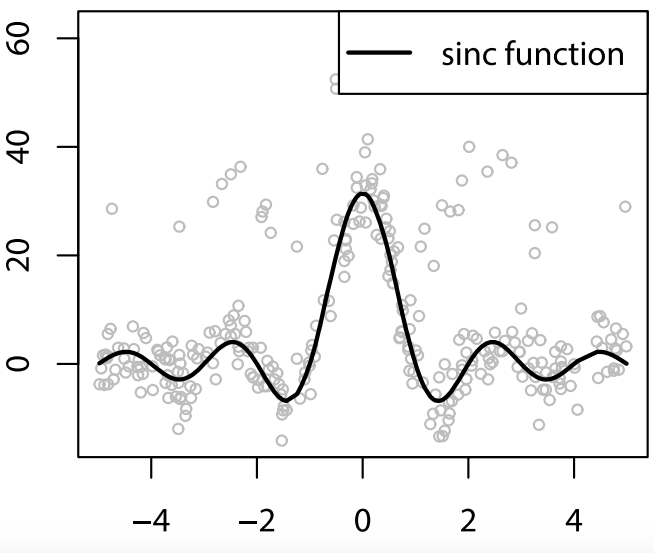
\includegraphics[height=0.6\textheight]{figures/sinc-fn-data}
\end{figure}

\let\thefootnote\relax\footnotetext{\tiny{From Natekin and Knoll's "Gradient boosting machines, a tutorial"}}
\end{frame}
%
\begin{frame}{Minimizing Square Loss with Ensemble of Decision Stumps}
\begin{center}
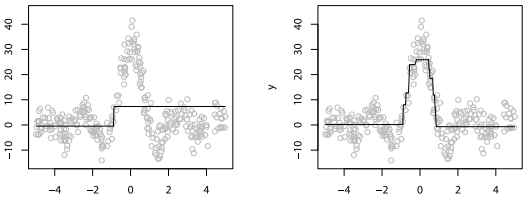
\includegraphics[height=0.3\textheight]{figures/sinc-fit-1step10steps}

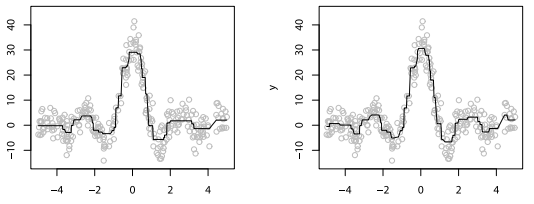
\includegraphics[height=0.3\textheight]{figures/sinc-fit-50steps100steps} 
\end{center}
Decision stumps with $1,10,50$, and $100$ steps, shrinkage $\lambda=1$.

\let\thefootnote\relax\footnotetext{\tiny{Figure 3 from Natekin and Knoll's "Gradient boosting machines, a tutorial"}}

\note[item]{A simple step function can be boosted to fit nonlinear data.}
\end{frame}
%

\section{Gradient Boosting in Practice}
\begin{frame}
{Prevent overfitting}
\begin{itemize}
\item Boosting is resistant to overfitting. Some explanations:
\begin{itemize}
\item Implicit feature selection: greedily selects the best feature (weak learner)
\item As training goes on, impact of change is localized.
\end{itemize}

\item But it can of course overfit. Common regularization methods:
\begin{itemize}
\item Shrinkage (small learning rate)
\item Stochastic gradient boosting (row subsampling)
\item Feature subsampling (column subsampling)
\end{itemize}
\end{itemize}
\end{frame}

\begin{frame}{Step Size as Regularization}

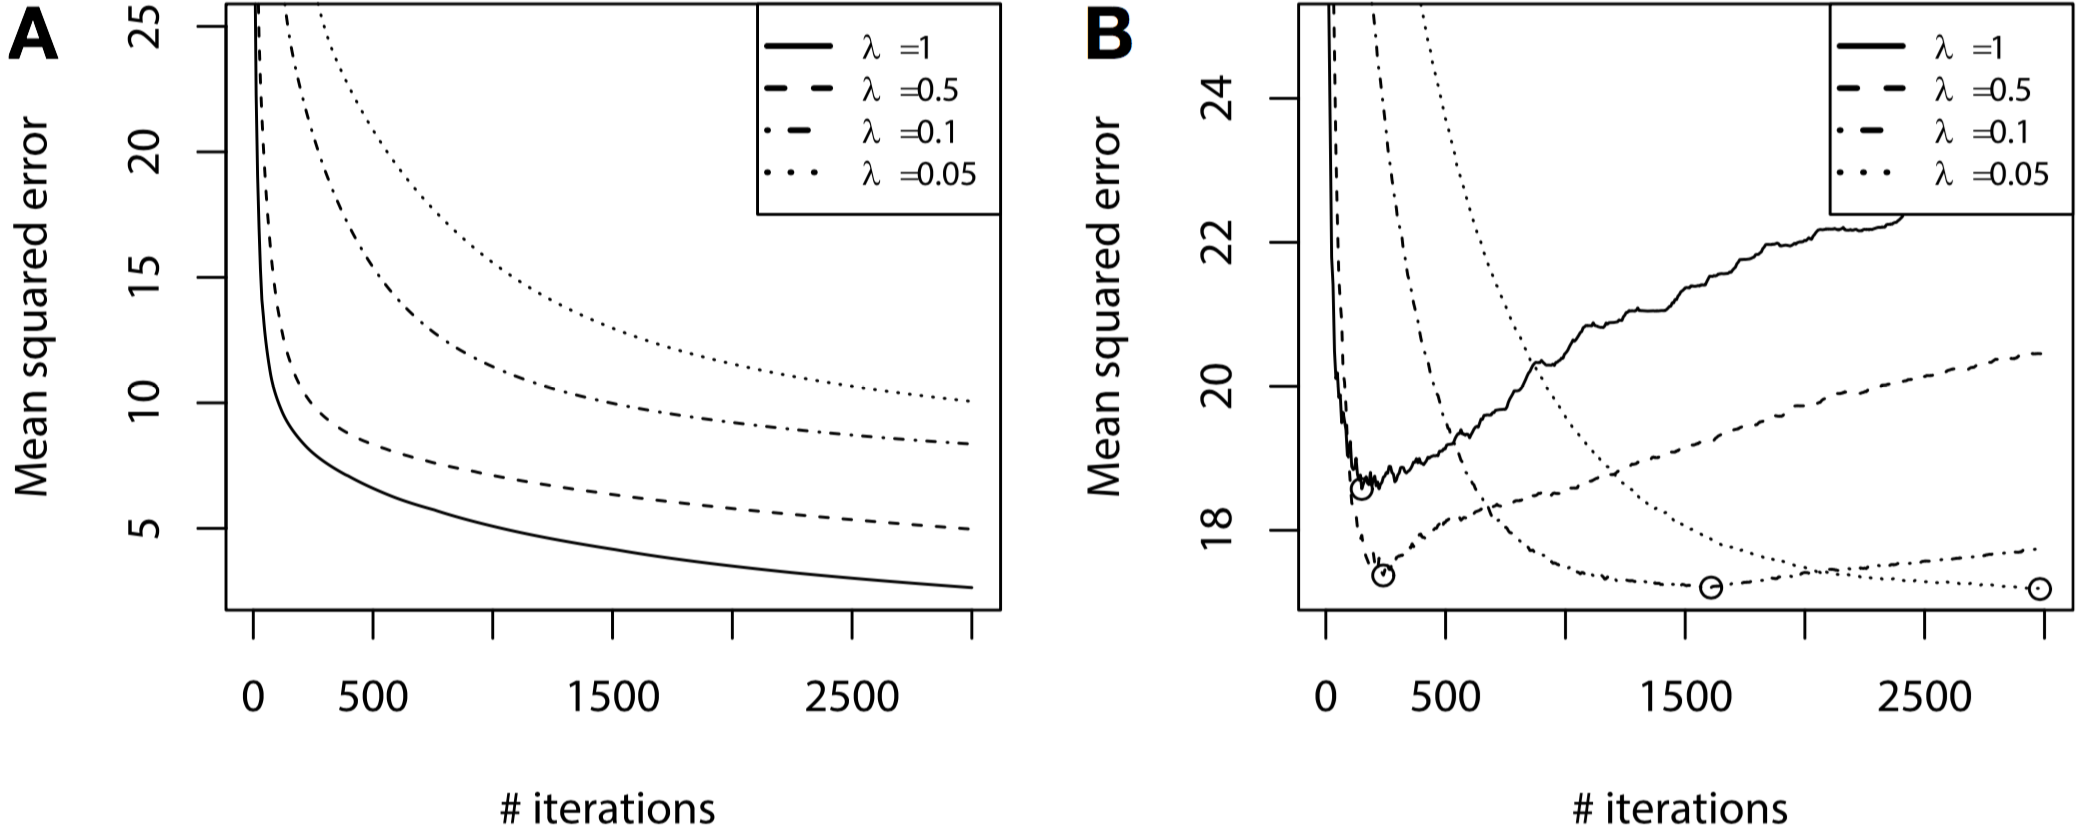
\includegraphics[width=0.8\textwidth]{figures/sinc-regression-train-validation} 

\begin{itemize}
\item (continued) sinc function regression
\item Performance vs rounds of boosting and shrinkage. (Left is training
set, right is validation set)
\end{itemize}

\let\thefootnote\relax\footnotetext{\tiny{Figure 5 from Natekin and Knoll's "Gradient boosting machines, a tutorial"}}
\note[item]{Left is training: larger step size leads to lower training loss as it updates more aggressively.}
\note[item]{Right is validation: larger step size converges faster but also converge to a worse solution.}
\end{frame}
%
\begin{frame}{Rule of Thumb}
\begin{itemize}
\item The smaller the step size, the more steps you'll need.
\item But never seems to make results worse, and often better.
\item So set your step size as small as you have patience for.
\end{itemize}
\note[item]{Next let's consider subsampling method.}
\end{frame}

\begin{frame}{Stochastic Gradient Boosting}
\begin{itemize}[<+->]
\item For each stage, 
\begin{itemize}[<.->]
\item choose random \emph{subset of data} for computing projected gradient step.
\end{itemize}
\item Why do this?
\begin{itemize}[<.->]
\item Introduce randomization thus may help overfitting.
\item Faster; often better than gradient descent given the same computation resource.
\end{itemize}
\item We can view this is a \textbf{minibatch method}. 
\begin{itemize}[<.->]
\item Estimate the ``true'' step direction
using a subset of data.
\end{itemize}
\let\thefootnote\relax\footnotetext{\tiny{Introduced by Friedman (1999) in \href{http://statweb.stanford.edu/~jhf/ftp/stobst.pdf}{Stochastic Gradient Boosting}. }}
\end{itemize}
\end{frame}
%
%\begin{frame}{Bag as Minibatch}
%\begin{itemize}
%\item Just as we argued for minibatch SGD, 
%\begin{itemize}
%\item sample size needed for a good estimate of step direction is independent
%of training set size
%\end{itemize}
%
%\pause{}
%\item Minibatch size should depend on 
%\begin{itemize}
%\item the complexity of base hypothesis space
%\item the complexity of the target function (Bayes decision function)
%\end{itemize}
%
%\pause{}
%\item Seems like an interesting area for both practical and theoretical
%pursuit.
%\end{itemize}
%\end{frame}
%

\begin{frame}{Column / Feature Subsampling}
\begin{itemize}
\item Similar to random forest, randomly choose \emph{a subset of features} for
each round.

\item XGBoost paper says: ``According to user feedback, using column sub-sampling
prevents overfitting even more so than the traditional row sub-sampling.''

\item Speeds up computation.
\end{itemize}
\end{frame}

%\begin{frame}{Newton Step Direction}
%\begin{itemize}
%\item For GBM, we find the closest $h\in\cf$ to the negative gradient
%\[
%-{\bf g}=-\del_{\vf}J({\bf f}).
%\]
%\item This is a ``first order'' method. 
%\end{itemize}
%
%\pause{}
%\begin{itemize}
%\item Newton's method is a ``second order method'':
%\begin{itemize}
%\item Find 2nd order (quadratic) approximation to $J$ at $\vf$.
%\begin{itemize}
%\item Requires computing gradient and Hessian of $J$.
%\end{itemize}
%\item Newton step direction points towards minimizer of the quadratic.
%\item Minimizer of quadratic is easy to find in closed form
%\end{itemize}
%
%\pause{}
%\item Boosting methods with projected Newton step direction:
%\begin{itemize}
%\item LogitBoost (logistic loss function)
%\item XGBoost (any loss \textendash{} uses regression trees for base classifier)
%\end{itemize}
%\end{itemize}
%\end{frame}
%%
%\begin{frame}{Newton Step Direction for GBM}
%\begin{itemize}
%\item Generically, second order Taylor expansion of $J$ at ${\bf f}$ in
%direction ${\bf r}$
%\[
%J({\bf f}+{\bf r})=J({\bf f})+\left[\del_{{\bf f}}J({\bf f})\right]^{T}{\bf r}+\frac{1}{2}{\bf r}^{T}\left[\del_{{\bf f}}^{2}J({\bf f})\right]{\bf r}
%\]
%
%
%\pause{}
%\item For $J({\bf f})=\sum_{i=1}^{n}\ell\left(y_{i},{\bf f}_{i}\right)$,
%\[
%J({\bf f}+{\bf r})=\sum_{i=1}^{n}\left[\ell\left(y_{i},{\bf f}_{i}\right)+g_{i}{\bf r}_{i}+\frac{1}{2}h_{i}{\bf r}_{i}^{2}\right],
%\]
%where $g_{i}=\partial_{{\bf f}_{i}}\ell\left(y_{i},{\bf f}_{i}\right)$
%and $h_{i}=\partial_{{\bf f}_{i}}^{2}\ell\left(y_{i},{\bf f}_{i}\right)$. 
%
%\pause{}
%\item Can find ${\bf r}$ that minimizes $J({\bf f}+{\bf r})$ in closed
%form. 
%
%\pause{}
%\item Can take step direction to be ``projection'' of ${\bf r}$ into
%base hypothesis space $\ch$.
%\end{itemize}
%\end{frame}

\begin{frame}
{Summary}
\begin{itemize}
\item Motivating idea of boosting: combine weak learners to produce a strong learner.
\item The statistical view: boosting is fitting an additive model (greedily).
\item The numerical optimization view: boosting makes local improvement iteratively---gradient descent in the function space.
\item Gradient boosting is a generic framework
\begin{itemize}
\item Any differentiable loss function
\item Classification, regression, ranking, multiclass etc.
\item Scalable, \eg XGBoost
\end{itemize}
\end{itemize}
\note[item]{We introduced boosting and Adaboost as an ensemble method in addition to bagging.}
\note[item]{But now we know that they are fundamentally very different ideas. The ensemble form of the final predictor is only a superficial connection.}
\note[item]{Boosting is fitting an additive model which aims to reduce bias, whereas often ensemble is meant to reduce variance.}
\note[item]{We can further generalize that to any loss function by functional gradient descent, or gradient boosting.}
\note[item]{In this lecture, we have seen how boosting started with a theoretical question and now produces large-scale system such as XGBoost used widely in practice. This is actually quite amazing.}
\end{frame}

\end{document}
